\section{Multiplicador binario \label{sec:s1}}

\begin{center}
	\begin{minipage}{12cm}
		\begin{tcolorbox}[title=Actividad 1]
			Completar el código del multiplicador binario para números de 8 bits en el lenguaje de su elección. Compilar y simular. Usando el \textit{Chip Planner}, verificar en donde se implementa el multiplicador por \textit{default} (elementos lógicos o hardware dedicado).
		\end{tcolorbox}	
	\end{minipage}
\end{center}

La visualización RTL del multiplicador binario en Verilog se muestra en la \autoref{fig:binary_multiplier_rtl}. Al momento de utilizar la herramienta de \textit{Chip Planner} se observa en la \autoref{fig:binary_multiplier_CP} que aparecen algunos elementos iluminados de azul, los cuales corresponden con el multiplicador. Si se acerca la imagen a uno de estos elementos (ver \autoref{fig:binary_multiplier_CPZoom}) se puede ver que el multiplicador fue implementado por la herramienta en hardware dedicado y esto se debe a que se identifico como un multiplicador, puesto que la descripción fue hecha por comportamiento, en caso de que se hubiera realizado por flujo de datos de bajo nivel, se habría implementado como elemento lógico. Finalmente, seleccionando uno de los elementos, se visualiza en la \autoref{fig:binary_multiplier_CPInside} uno de los elementos del multiplicador. 

Las simulaciones para el código en Verilog se visualizan en la \autoref{fig:binary_multiplier_WaveBi} en base binaria y en la \autoref{fig:binary_multiplier_WaveDe} en base decimal. Cabe resaltar que los valores utilizados para los bancos de pruebas fueron obtenidos de un generador de números aleatorios entre 0 y 255 \cite{numeros_2024}.

\begin{figure}[ht]
	\centering
	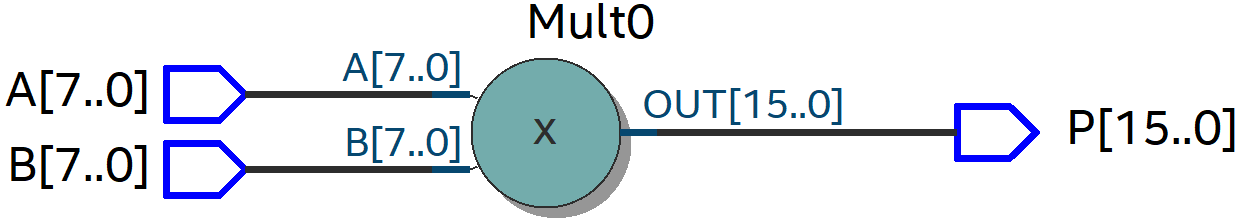
\includegraphics[scale=0.5]{Binary_Multiplier_RTL.png}
	\caption{Diagrama RTL del multiplicador binario de 8 bits. \label{fig:binary_multiplier_rtl}}
\end{figure}

\begin{figure}[ht]
	\centering
	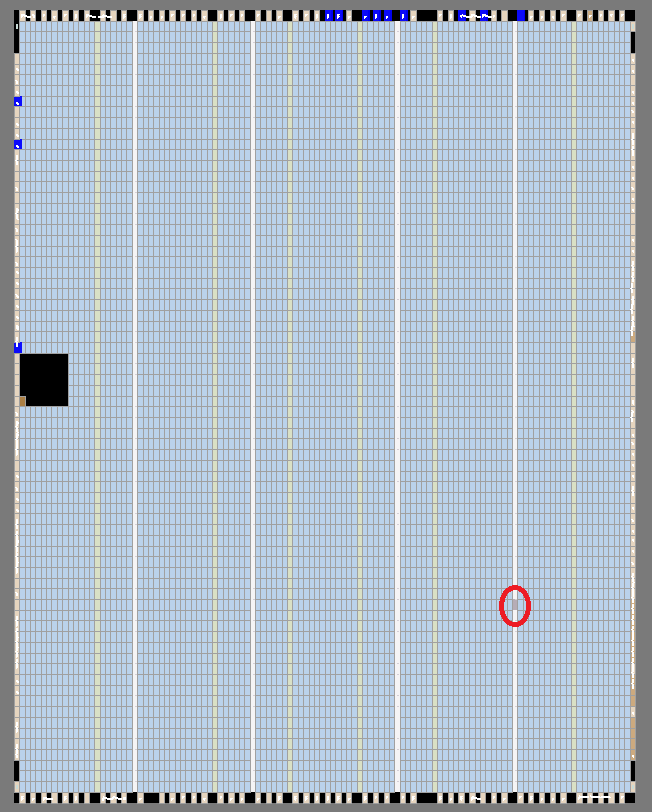
\includegraphics[scale=0.55]{Binary_Multiplier_CP.png}
	\caption{Vista de la herramienta de \textit{Chip Planner} del multiplicador binario. \label{fig:binary_multiplier_CP}}
\end{figure}

\begin{figure}[ht]
	\centering
	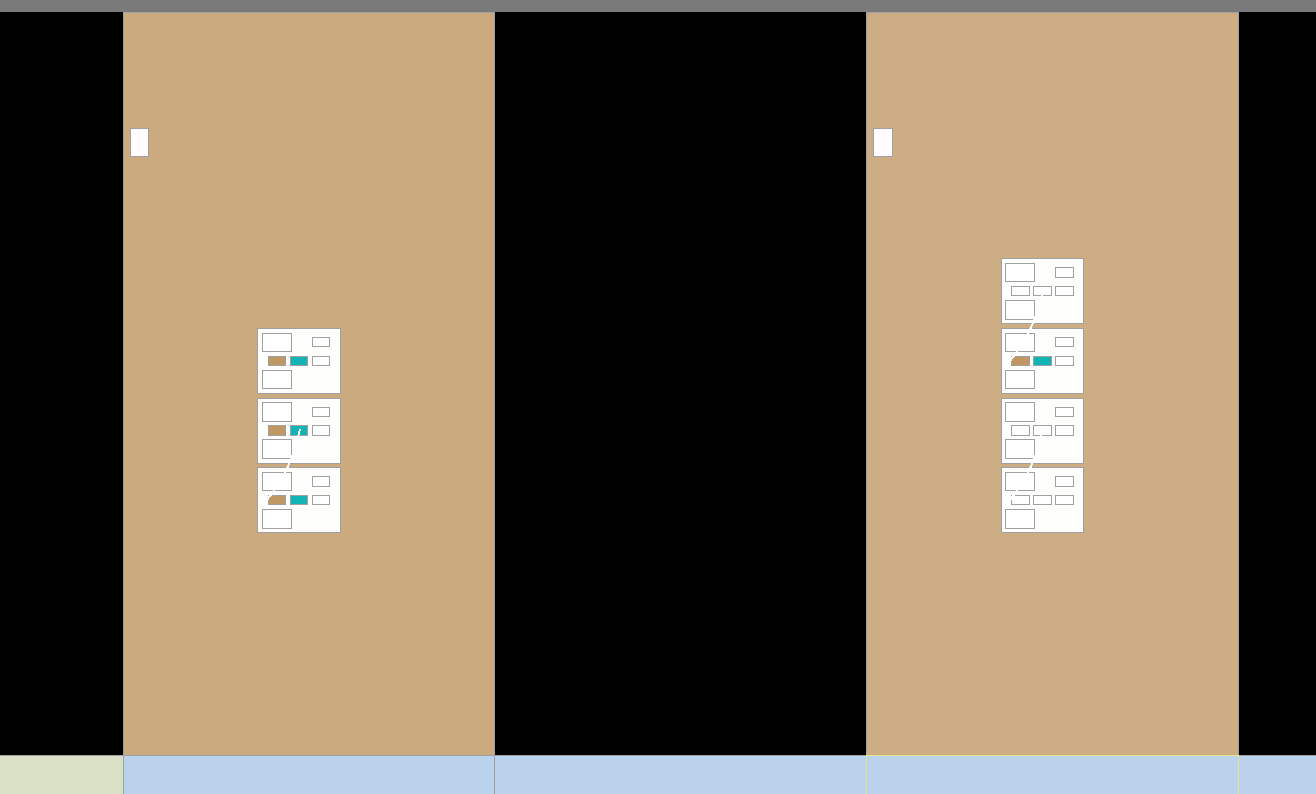
\includegraphics[scale=0.4]{Binary_Multiplier_CPZoom.png}
	\caption{Vista de la herramienta de \textit{Chip Planner} del multiplicador binario (acercamiento). \label{fig:binary_multiplier_CPZoom}}
\end{figure}

\begin{figure}[ht]
	\centering
	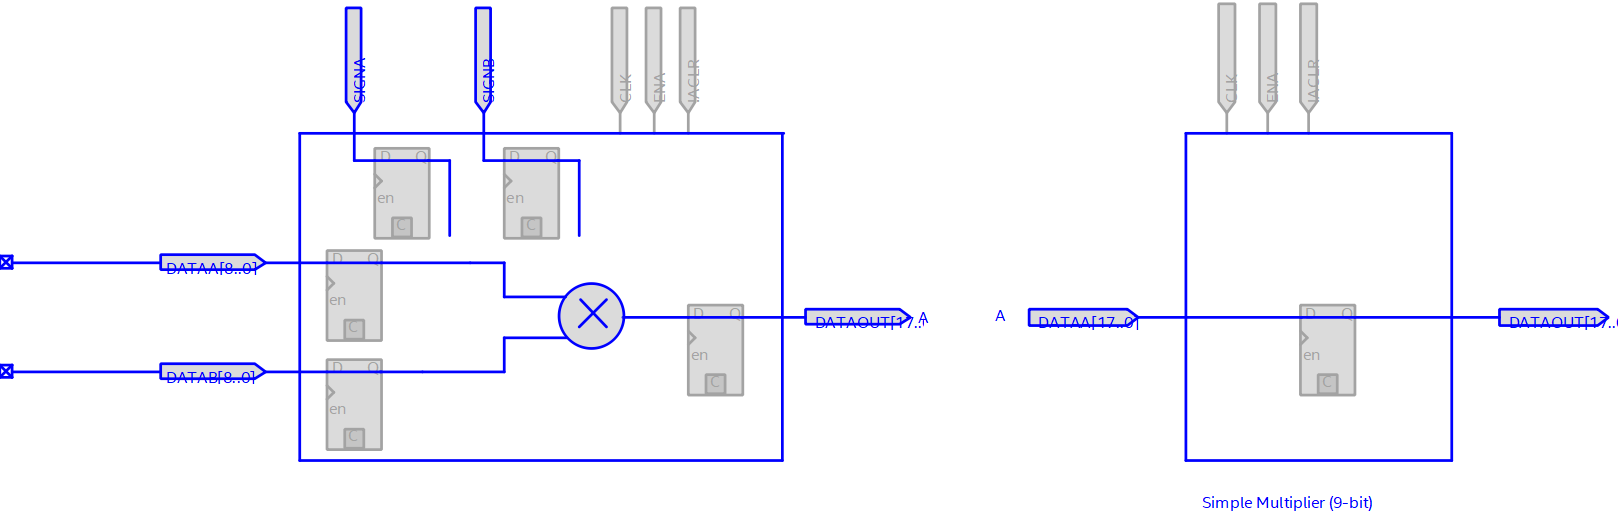
\includegraphics[scale=0.6]{Binary_Multiplier_CPInside.png}
	\caption{Vista de un elemento de hardware dedicado del multiplicador binario. \label{fig:binary_multiplier_CPInside}}
\end{figure}

\begin{figure}[ht]
	\centering
	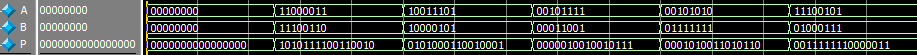
\includegraphics[scale=0.7]{Binary_Multiplier_WaveBi.png}
	\caption{Simulación del multiplicador binario con el visor de formas de onda de ModelSim (Base binaria). \label{fig:binary_multiplier_WaveBi}}
\end{figure}

\begin{figure}[ht]
	\centering
	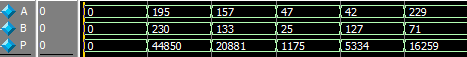
\includegraphics[scale=1.3]{Binary_Multiplier_WaveDe.png}
	\caption{Simulación del multiplicador binario con el visor de formas de onda de ModelSim (Base decimal). \label{fig:binary_multiplier_WaveDe}}
\end{figure}
